\subsection{Fourier Series}
\subsubsection{Real Fourier Series}
We can express functions using an infinite basis of orthogonal functions. One very prominent set of orthogonal functions is sinusoidal functions.\\
We can express functions as a sum of sines and cosines of different frequencies. This is known as the \textit{Fourier series}.\\
The Fourier series will be of the form
$$f(x)=\sum_{n=0}^\infty a_n\cos\brround{\frac{n\pi x}{L}}+\sum_{n=1}^\infty b_n\sin\brround{\frac{n\pi x}{L}}=a_0+\sum_{n=1}^\infty\brround{a_n\cos\brround{\frac{n\pi x}{L}}+b_n\sin\brround{\frac{n\pi x}{L}}}$$
To match functions, we can use the concept of orthogonality.\\
$f(x)$ and $g(x)$ are orthogonal if $\displaystyle{\int_{-L}^Lf(x)g(x)dx=0}$\\
Trig functions have some particularly useful orthogonality properties.\\
For where $m,n\in\N$
\begin{align*}
    &\int_{-L}^L\sin\brround{\frac{n\pi x}{L}}\sin\brround{\frac{m\pi x}{L}}dx=\eqnsystem{0 & \text{if }m\neq n\\ L & \text{if }m=n}\\
    &\int_{-L}^L\cos\brround{\frac{n\pi x}{L}}\cos\brround{\frac{m\pi x}{L}}dx=\eqnsystem{0 & \text{if }m\neq n\\ L & \text{if }m=n\neq 0\\ 2L & \text{if }m=n=0}\\
    &\int_{-L}^L\sin\brround{\frac{n\pi x}{L}}\cos\brround{\frac{m\pi x}{L}}dx=0
\end{align*}
Not all functions will have a Fourier series. In order to determine if the function has a Fourier series, it must satisfy the following criteria:
\begin{itemize}
    \item Is single-valued
    \item Is absolutely integrable
    \[ \int_T|f(x)|dx<\infty \]
    \item Has a finite number of maxima and minima
    \item Has a finite number of discontinuities
\end{itemize}
The Fourier series will converge to $f(x)$ where $f(x)$ is continuous and half the value of the jump where it's discontinuous.\\

So far, we have introduced what Fourier series is; now let's get into how to use it.\\
When using Fourier series, we are trying to solve for the unknown coefficients, $a_0,a_m,b_m$ in the series.\\
We can make use of the trig orthogonality rules we determined earlier to determine these coefficients.\\
To solve for $b_m$, we can multiply by $\sin\brround{\frac{m\pi x}{L}}$ and integrate from $-L$ to $L$.
\begin{align*}
    &f(x)=\sum_{n=0}^\infty a_n\cos\brround{\frac{n\pi x}{L}}+\sum_{n=1}^\infty\sin\brround{\frac{n\pi x}{L}}\\
    &\int_{-L}^L f(x)\sin\brround{\frac{m\pi x}{L}}dx=\sum_{n=0}^\infty a_n\underbrace{\int_{-L}^L\cos\brround{\frac{n\pi x}{L}}\sin\brround{\frac{m\pi x}{L}}dx}_{=0}+\sum_{n=1}^\infty b_n\underbrace{\int_{-L}^L\sin\brround{\frac{n\pi x}{L}}\sin\brround{\frac{m\pi x}{L}}dx}_{=L\text{ if }m=n}\\
    &\int_{-L}^Lf(x)\sin\brround{\frac{m\pi x}{L}}dx=b_mL\\
    &b_m=\frac{1}{L}\int_{-L}^L f(x)\sin\brround{\frac{m\pi x}{L}}dx
\end{align*}
To find $a_m$, we do the same thing but multiply by $\cos\brround{\frac{m\pi x}{L}}$
\begin{align*}
    &f(x)=\sum_{n=0}^\infty a_n\cos\brround{\frac{n\pi x}{L}}+\sum_{n=1}^\infty\sin\brround{\frac{n\pi x}{L}}\\
    &\int_{-L}^Lf(x)\cos\brround{\frac{m\pi x}{L}}dx=\sum_{n=0}^\infty a_n\underbrace{\int_{-L}^L\cos\brround{\frac{n\pi x}{L}}\cos\brround{\frac{m\pi x}{L}}dx}_{=\eqnsystem{2L & \text{if }m=0\\ L & \text{if }m=n}}+\sum_{n=1}^\infty b_n\underbrace{\int_{-L}^L\sin\brround{\frac{n\pi x}{L}}\sin\brround{\frac{m\pi x}{L}}dx}_{=0}\\
    &a_0=\frac{1}{2L}\int_{-L}^L f(x)dx\\
    &a_m=\frac{1}{L}\int_{-L}^L f(x)\cos\brround{\frac{m\pi x}{L}}dx
\end{align*}
If $f(x)$ is odd then
\begin{align*}
    &a_0=a_m=0\\
    &b_m=\frac{2}{L}\int_0^L f(x)\sin\brround{\frac{m\pi x}{L}}dx
\end{align*}
If $f(x)$ is even then
\begin{align*}
    &b_m=0\\
    &a_0=\frac{1}{L}\int_0^L f(x)dx\\
    &a_m=\frac{2}{L}\int_0^L f(x)\cos\brround{\frac{m\pi x}{L}}dx
\end{align*}
If you are trying to match a function that is only defined between $0$ and $L$ then you must make an odd or even extension.\\
Ex: for the function $1-x$ defined on $0\leq x\leq1$, the even extension would be
\begin{align*}
    &f^e(x)=\eqnsystem{1-x & x\geq 0\\ x+1 & x<0}
\end{align*}
The odd extension would be
\begin{align*}
    &f^e(x)=\eqnsystem{1-x & x>0\\ 0 & x=0\\ -1-x & x<0}
\end{align*}
Note that when there is a discontinuity, the function will take the average value of the limit from both sides, hence why $f^e(x)=0$ for where $x=0$ as we have
\begin{align*}
    &f^e(0)=\frac{1}{2}\brround{\lim_{x\to 0^-}f^e(x)+\lim_{x\to0^+}f^e(x)}=\frac{1}{2}\brround{-1+1}=0
\end{align*}
When dealing with a function that is neither even or odd, we will have to use the full Fourier series with both sines and cosines.\\

Ex: Find the Fourier series of a square wave defined by
\begin{align*}
    &f(x)=\eqnsystem{1 & 0<t<\pi\\ -1 & \pi<t<2\pi}
\end{align*}
\centerline{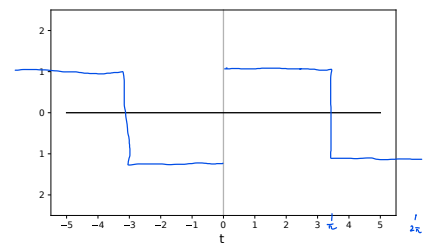
\includegraphics[scale=1]{Images/FourierImages/SeriesEx2.png}}
The odd extension is drawn above and given that this is an odd function we can express it using only sine terms.
\begin{align*}
    &2L=2\pi\Ra L=\pi\\
    &b_n=\frac{2}{\pi}\int_0^\pi f(x)\sin\brround{nx}dx=\frac{2}{\pi}\int_0^\pi\sin(nx)dx=-\frac{2\cos(nx)}{n\pi}\eval_0^\pi\\
    &b_n=\frac{2}{n\pi}(-\cos(n\pi)+1)=\frac{2}{n\pi}(-(-1)^n+1)\\
    &b_n=\frac{4}{n\pi},\text{ for odd $n$}\\
    &b_n=0,\text{ for even $n$}\\
    &f(x)=\sum_{n=1}^\infty\frac{4}{n\pi}\sin(nx),\ n=\brcurly{1,3,5,\ldots}
\end{align*}
We can also rewrite this as $n=2k+1$ if we choose
\begin{align*}
    &f(x)=\sum_{k=0}^\infty\frac{4}{(2k+1)\pi}\sin((2k+1)x)
\end{align*}
This function only has odd values of $n$ so it is considered to only contain what's called odd harmonics.\\

The even harmonics of the system correspond to even $n$ and require
$$f\brround{t+\frac{T}{2}}=f(t)$$
The odd harmonics correspond to odd $n$ and require
$$f\brround{t+\frac{T}{2}}=-f(t)$$
\subsubsection{Complex Fourier Series}
For functions that are neither even or odd, this process of finding 3 coefficients through integration may seem a little messy and it turns out that there is a nicer way to express the Fourier series using complex numbers:\\
Right now we have
\begin{align*}
    &f(\alpha)=a_0+\sum_{n=1}^\infty a_n\cos(n\alpha)+\sum_{n=1}^\infty\sin(n\alpha)
\end{align*}
We can make use of the identities
\begin{align*}
    &\cos\theta=\frac{e^{i\theta}+e^{-i\theta}}{2},\ \sin\theta=\frac{e^{i\theta}-e^{-i\theta}}{2}
\end{align*}
So we have
\begin{align*}    
    &f(\alpha)=a_0+\sum_{n=1}^\infty\frac{a_n}{2}\brround{e^{in\alpha}+e^{-in\alpha}}+\sum_{n=1}^\infty\frac{b_n}{2}\brround{e^{in\alpha}-e^{-in\alpha}}\\
    &f(\alpha)=\sum_{n=1}^\infty\brround{\frac{a_n-ib_n}{2}}e^{in\alpha}+\sum_{n=1}^\infty\brround{\frac{a_n+ib_n}{2}}e^{-in\alpha}\\
    &f(\alpha)=\underbrace{a_0}_{c_0}+\sum_{n=1}^\infty\underbrace{\brround{\frac{a_n-ib_n}{2}}}_{c_n}e^{in\alpha}+\sum_{n=-\infty}^{-1}\underbrace{\brround{\frac{a_{-n}+ib_{-n}}{2}}}_{c_n}e^{in\alpha}\\
    &f(\alpha)=\sum_{n=-\infty}^\infty c_ne^{in\alpha},\ c_n=\frac{1}{2L}\int_{-L}^Lf(\alpha)e^{-in\alpha}d\alpha
\end{align*}
This is a more elegant way of expressing the Fourier series and gives rise to more applications. Expressing the Fourier series using sines and cosines may be easier to use in application when dealing with real functions as it will give real functions as outputs, avoiding the issue of converting between real and complex functions. For the remainder of this section, however, we will focus on the complex version of the Fourier series and express it as
$$\boxed{x(t)=\sum_{k=-\infty}^\infty c_ke^{ik\omega t}}$$
$\omega$ represents the fundamental frequency of the function where
$$\omega=\frac{2\pi}{T}$$
If $x(t)$ is a real function then the negative coefficients are complex conjugates of the positive coefficients.
\begin{align*}
    &\text{for real functions, }x(t)=\overline{x(t)}\\
    &\sum_{k=-\infty}^\infty c_ke^{ik\omega t}=\sum_{k=-\infty}^\infty \overline{c_k}e^{-ik\omega t}=\sum_{k=-\infty}^\infty c_{-k}e^{ik\omega t}
\end{align*}
In order to evaluate these coefficients, we can multiply both sides of the function by $e^{-im\omega t}$ and then integrating.
\begin{align*}
    &e^{-im\omega t}x(t)=\sum_{k=-\infty}^\infty c_ke^{i\omega t(k-m)}\\
    &\frac{1}{T}\int_Tx(t)e^{-im\omega t}dt=\frac{1}{T}\int_T\sum_{k=-\infty}^\infty c_ke^{i\omega t(k-m)}dt
\end{align*}
Case: $k\neq m$:
\begin{align*}
    &\frac{1}{T}\int_Tx(t)e^{-im\omega t}dt=\frac{1}{T}\int\cos((k-m)\omega t)dt+\frac{j}{T}\int_T\sin((k-m)\omega t)dt=0
\end{align*}
Case: $k=m$:
\begin{align*}
    &\frac{1}{T}\int_T x(t)e^{-im\omega t}dt=\frac{1}{T}\int_T c_mdt=c_m
\end{align*}
And so we get the coefficients as
$$\boxed{c_k=\frac{1}{T}\int_T x(t)e^{-ik\omega t}dt}$$
Ex: Find the Fourier series of $e^{-t}$ for $-1\leq t\leq 1$\\
\centerline{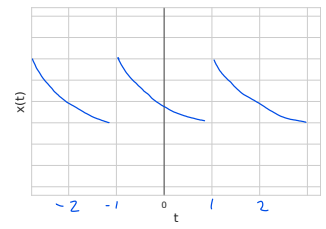
\includegraphics[scale=1.1]{Images/FourierImages/SeriesEx1.png}}
\begin{align*}
    &T=2,\ \omega=\frac{2\pi}{T}=\pi\\
    &c_k=\frac{1}{2}\int_{-1}^1 e^{-t}e^{-ik\pi t}dt\\
    &c_k=\frac{1}{2}\int_{-1}^1e^{t(1+i\pi k)}dt\\
    &c_k=\frac{1}{2(1+i\pi k)}e^{t(1+i\pi k)}\eval_{-1}^1\\
    &c_k=\frac{1}{2(1+i\pi k)}\brround{e^{1+i\pi k}-e^{-(1+i\pi k)}}\\
    &c_k=\frac{(-1)^k}{2(1+i\pi k)}\brround{e-e^{-1}}\\
    &x(t)=\sum_{k=-\infty}^\infty \frac{(-1)^k}{2(1+i\pi k)}\brround{e-e^{-1}}e^{i\pi kt}
\end{align*}

If we decide to truncate the Fourier series (evaluate between $-N$ and $N$ instead of $-\infty$ and $\infty$) then we get the error in the approximation is
$$e_N=x(t)-x_N(t)=x(t)-\sum_{k=-N}^N c_ke^{jk\omega t}$$
and the error over one period is
$$E_N=\int_T|e_N(t)|^2dt$$
This also happens to be the energy of the error. The energy of a signal over a period is given by
$$\langle E\rangle =\int_T|x(t)|^2dt$$
and the power over a period is given by
$$P=\frac{\langle E\rangle}{T}=\frac{1}{T}\int_T|x(t)|^2dt$$
Using Parseval's relation, we can also express the power in terms of the coefficients:
$$P=\frac{1}{T}\int_T|x(t)|^2dt=\sum_{k=-\infty}^\infty|c_k|^2$$


\subsubsection{Discrete Fourier Transform}
In many real-world applications the data that we are working with may not be processed as a continuous-time signal, but rather as a discrete-time signal instead. If we want to apply the same tricks to work with this data as we did in continuous time, we will require a discrete-time representation of the Fourier series.\\
First we must note that because of the integer values, there will be more conditions on periodicity of a function. Because $n$ can only be integer values, the period, $N$, cannot be a fraction.\\
A periodic function can be written as $e^{i\omega n}$. If the function has period $N$ then this means that
\[ e^{i\omega (n+N)}=e^{i\omega n} \]
This implies that $e^{i\omega N}=1$. So then we can get
\[ \omega N=2\pi m,\ m\in\Z \]
This means that $\frac{\omega}{2\pi}$ must be rational in order for the function to be periodic.\\
If we take the function $x=\cos(3n)$ it is an example of a non-periodic function which is a little counterintuitive but it's because $\frac{\omega}{2\pi}$ is not a rational number and so the value of $x[n]$ will jump around within the range of $\cos(3n)$ but never quite repeat in a periodic manner.\\
If we take $x=\cos(\pi n)$, however, we can see that the frequency is $\omega=\pi$ and so $\frac{\omega}{2\pi}=\frac{1}{2}\in\Q$ which implies the function is periodic. If you plot the values of both of these functions in discrete time, you'll see that this is true.\\
Because of these limitations, the smallest possible period we can get is $N=1$ which corresponds to a largest possible frequency of $\omega=2\pi$ so our frequency will always be in the range of
$$0\leq\omega\leq 2\pi$$
Ex: Find the fundamental period of $x[n]=\cos\brround{\frac{5\pi}{6}n}$.\\
The period is given by $T=\frac{2\pi}{\omega}=\frac{12}{5}$. If we keep repeating the period, the first integer value is $5T=5\cdot\frac{12}{5}=12=N$. This corresponds to the fundamental period of the function.\\

With the conditions of periodic functions out of the way, we can go into how we can express the discreet-time Fourier series. Similar to the continuous-time case, we will have a basis that is comprised of complex exponential functions of different frequencies. Each of these different frequencies are called harmonics. By summing them we can an expression that will be our discrete Fourier series.
$$\boxed{x[n]=\sum_{k=0}^{N-1}c_ke^{ik\frac{2\pi n}{N}}}$$
Once again, we can make the argument that the complex exponential basis of the Fourier series forms an orthogonal basis and we can make use of its orthogonality properties to get the $c_k$ values
$$\boxed{c_k=\frac{1}{N}\sum_{n=0}^{N-1}x[n]e^{-i\frac{2\pi n}{N}}}$$

\subsubsection{Fourier Transform}
So far we have found a nice way of expressing periodic functions using the Fourier series but what if we wanted to generalize this to aperiodic functions. We can make use of a powerful tool called the Fourier transform. It is a generalization of the Fourier series. Let's look at this through an example.\\
The following function is described by
\[ x(t)=\eqnsystem{1 & |t|<T_1\\ 0 & T_1<|t|<\frac{T}{2}} \]
\centerline{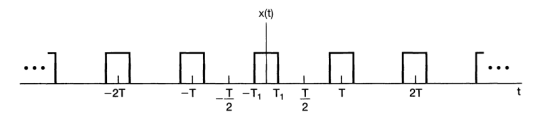
\includegraphics[scale=1]{Images/FourierImages/FourierTransformDerivation.png}}
We can compute its Fourier coefficients as
\begin{align*}
    &c_k=\frac{1}{T}\int_{-T/2}^{T/2}x(t)e^{-i\omega kt}dt\\
    &c_k=\frac{1}{T}\int_{-T_1}^{T_1}e^{-ik\omega t}dt=-\frac{e^{-ik\omega t}}{ik\omega}\eval_{-T_1}^{T_1}=\frac{1}{ik\omega}\brround{e^{ik\omega T_1}-e^{-ik\omega T_1}}\\
    &c_k=\frac{2\sin(k\omega T_1)}{k\omega T}
\end{align*}
\centerline{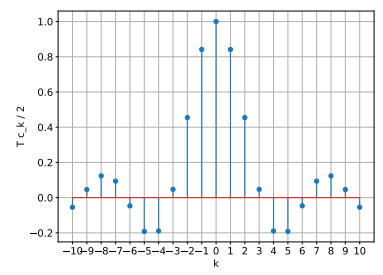
\includegraphics[scale=1]{Images/FourierImages/DTSincEx1.png}}
The Fourier coefficients (plotted above) output the discrete case of what is commonly called the sinc function which is proportional to
$$\mathrm{sinc}(x)=\frac{\sin(x)}{x}$$
Right now we only have information about integer values of $k$ but what if we extrapolate this graph
\centerline{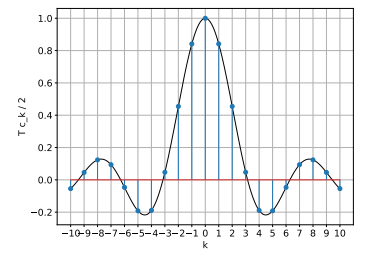
\includegraphics[scale=1]{Images/FourierImages/CTSincEx1.png}}
This gives us a continuous function of the $k$ values
\[ f(k\omega)=\eqnsystem{1 & k=0\\ \frac{\sin(k\omega T_1)}{k\omega} & k\neq 0} \]
We can then express the $c_k$ values as
\[ c_k=\frac{2}{T}f(k\omega) \]
Now what if we take our periodic square wave and make $T$ very large. This would have the effect of separating and isolating each periodic part of the function so that it resembles an apeariodic function.\\
We know $\omega=\frac{2\pi}{T}$ so as $T$ grows, $\omega$ will become very small. This will have the effect of squishing the $k\omega$ steps closer and closer together.\\
\centerline{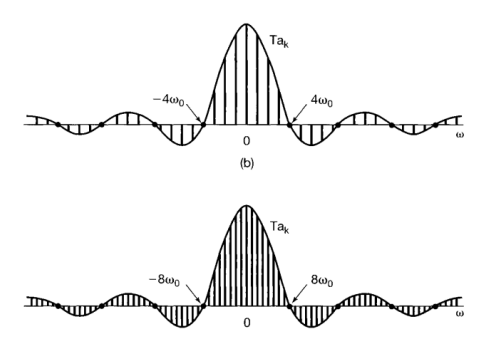
\includegraphics[scale=1]{Images/FourierImages/convergingSinc.png}}
This gives rise to the following relation
\begin{align*}
    &x(t)=\sum_{k=-\infty}^\infty c_ke^{ik\omega t}\\
    &\text{as }T\to\infty,\ \omega\to 0\\
    &x(t)\approx\int_{-\infty}^\infty c_ke^{i\omega t}d\omega
\end{align*}
And so then
\begin{align*}
    &c_k=\frac{1}{T}\int_{-T/2}^{T/2}x(t)e^{-ik\omega t}dt\\
    &\text{as }T\to\infty\\
    &c_k=\frac{1}{T}\int_{-\infty}^\infty x(t)e^{-i\omega t}dt
\end{align*}
Let us define
$$X(i\omega)=\int_{-\infty}^\infty x(t)e^{-i\omega t}dt$$
so that
$$c_k=\frac{1}{T}X(i\omega)$$
If we go back to the Fourier series we get
\begin{align*}
    &x(t)=\sum_{k=-\infty}^\infty \frac{1}{T}X(i\omega)e^{ik\omega t}\\
    &T=\frac{2\pi}{\omega}\\
    &x(t)=\frac{1}{2\pi}\sum_{k=-\infty}^\infty X(i\omega)e^{ik\omega t}\omega\\
    &\text{as }T\to\infty,\ \omega\to d\omega,\ k\omega\to \omega\\
    &x(t)=\frac{1}{2\pi}\int_{-\infty}^\infty X(i\omega)e^{i\omega t}d\omega
\end{align*}

This derivation gives a very important result giving the Fourier transform, defined as
$$\boxed{X(i\omega)=\int_{-\infty}^\infty x(t)e^{-i\omega t}dt}$$
and the inverse Fourier transform given by
$$\boxed{x(t)=\frac{1}{2\pi}\int_{-\infty}^\infty X(i\omega)e^{i\omega t}}$$

The Fourier transform is denoted as
$$X(i\omega)=\F\brcurly{x(t)}$$
and the inverse Fourier transform is written as
$$x(t)=\F^{-1}\brcurly{X(i\omega)}$$
The Fourier transform is a linear operation which means that
$$\F\brcurly{ax(t)+by(t)}=aX(i\omega)+bY(i\omega)$$
It will have the time shifting identity
$$\F\brcurly{x(t-t_0)}=e^{-i\omega t_0}X(i\omega)$$
It will have the conjugation property
$$\F\brcurly{\overline{x(t)}}=\overline{X(-i\omega)}$$
Time scaling is given by
$$\F\brcurly{x(at)}=\frac{1}{|a|}X\brround{\frac{i\omega}{a}}$$
Differentiation is given by
$$\F\brcurly{\ddx[x(t)]{t}}=i\omega X(i\omega)$$

Ex: Find the Fourier transform of $x(t)=e^{-at}u(t)$
\begin{align*}
    &X(i\omega)=\int_{-\infty}^\infty x(t)e^{-i\omega t}dt=\int_0^\infty e^{-at}e^{-i\omega t}dt\\
    &=\int_0^\infty e^{-(a+i\omega)t}dt=\frac{-1}{a+i\omega}\eval_0^\infty=\frac{1}{a+i\omega}
\end{align*}
Ex2: Find the Fourier transform of $\frac{d^2}{dx^2}x(t-1)$
\[ \F\brcurly{\frac{d^2}{dx^2}x(t-1)}=-\omega^2e^{-i\omega}X(i\omega) \]


\subsubsection{Frequency Responses}
If we go back to convolution, we will see that the convolution has many applications to the Fourier series and transform.\\
If we have $x(t)=e^{j\omega t}$ then it will be an eigenfunction of the convolution operation.
\begin{align*}
    y(t)&=\int_{-\infty}^\infty x(t-\tau)h(\tau)d\tau=\int_{-\infty}^\infty e^{j\omega(t-\tau)}h(\tau)d\tau\\
    &=e^{i\omega t}\int_{-\infty}^\infty e^{-i\omega \tau}h(\tau)d\tau\\
    &=e^{i\omega t}H(i\omega)
\end{align*}
where $H(j\omega)$ is called the frequency response of the system.\\
This eigenfunction, $e^{j\omega t}$, will have an infinite number of harmonics, expressed as $e^{j\omega kt}=e^{jk\frac{2\pi}{T}t}$.\\
If we write a linear combination of all these eigenfunctions, we get the Fourier series.
$$x(t)=\sum_{k=-\infty}^\infty c_ke^{jk\omega t}$$
Combining this with the frequency response, we can express a signal as a Fourier series times a frequency response
$$y(t)=\sum_{k=-\infty}^\infty c_kH(i\omega)e^{jk\omega t}$$
From the start of the above derivation, this is just the same as
$$y(t)=x(t)*h(t)$$
where
$$H(i\omega)=\F\brcurly{h(t)}$$
Note that if we take $x(t)=\delta(t)$ then we get that
$$y(t)=\delta(t)*h(t)=h(t)$$
so $y(t)=h(t)$ when $x(t)=\delta(t)$. $h(t)$ is called the impulse response of a system.\\
The frequency response can be used to easily compute the output signal
$$x(t)\to y(t)=\sum_{k=-\infty}^\infty c_kH(j\omega)e^{jk\omega t}$$
$$x[n]\to y[n]=\sum_{k=0}^{N-1}c_k H(e^{jk\omega})e^{jk\omega n}$$
A very nice property of the Fourier transform is how it treats convolution. Convolution in the time-domain corresponds to multiplication in the frequency domain.
$$\boxed{\F\brcurly{x(t)*h(t)}=X(i\omega)H(i\omega)}$$
Using these relationships along with the Fourier transform, we are able to find the output of a given signal in both the time and frequency domain, allowing us do do our computations in either domain.\\
Ex: Given $x(t)=e^{-t}u(t)$ and $h(t)=e^{t}u(-t)$, find $y(t)$.
\begin{align*}
    &\F\brcurly{e^{-t}u(t)}=\frac{1}{1+i\omega}=X(i\omega)\\
    &\F\brcurly{x(t)}=X(-i\omega)\Ra \F\brcurly{e^{at}u(-t)}=\frac{1}{1-i\omega}=H(i\omega)\\
    &Y(i\omega)=X(i\omega)H(i\omega)=\frac{1}{(1+i\omega)(1-i\omega)}\\
    &Y(i\omega)=\frac{A}{1+i\omega}+\frac{B}{1-i\omega}\\
    &\eqnsystem{A+B=1\\ B-A=0}\Ra A=B\Ra 2A=1\Ra A=B=\frac{1}{2}\\
    &Y(i\omega)=\frac{1/2}{1+i\omega}+\frac{1/2}{1-i\omega}\\
    &y(t)=\F^{-1}\brcurly{Y(i\omega)}=\frac{1}{2}x(t)+\frac{1}{2}h(t)\\
    &y(t)=\frac{1}{2}e^{-t}u(t)+\frac{1}{2}e^tu(-t)\\
    &y(t)=\frac{1}{2}e^{-|t|}
\end{align*}
Given an ordinary differential equation, we can find the frequency response of the system using the differentiation property.\\
Ex: $y'''-4y'=3x''+x$\\
We can start by taking the Fourier transform of both sides
\begin{align*}
    &(i\omega)^3Y(i\omega)-4(i\omega)Y(i\omega)=3(i\omega)^2X(i\omega)+X(i\omega)\\
    &Y=XH\Ra H=\frac{Y}{X}\\
    &H=\frac{1-\omega^2}{-i\omega^3-4i\omega}=\frac{1-\omega^2}{i\omega(i\omega+2)(i\omega-2)}\\
    &H=\frac{A}{i\omega}+\frac{B}{i\omega+2}+\frac{C}{i\omega-2}\\
    &H(i\omega)=-\frac{1}{4}\frac{1}{i\omega}+\frac{13}{8}\frac{1}{i\omega+2}+\frac{13}{8}\frac{1}{i\omega-2}
\end{align*}
We can also express the Fourier transform in polar form:
$$X(i\omega)=|X(i\omega)|e^{i\angle X(i\omega)}$$
Combining this with the relationship $Y(i\omega)=X(i\omega)H(i\omega)$ we can get
\[ |Y(i\omega)|e^{\angle Y(i\omega)}=|X(i\omega)|e^{i\angle X(i\omega)}|H(i\omega)|e^{i\angle H(i\omega)} \]
We can make use of the magnitude and phase of the input and outputs to solve for the frequency response.
$$|H(i\omega)|=\frac{|Y(i\omega)|}{|X(i\omega)|}$$
and
$$\angle H(i\omega)=\angle Y(i\omega)-\angle X(i\omega)$$
Ex: What is the magnitude and phase of the frequency response for $y(t)=x(t)+x'(t)$?
\begin{align*}
    &Y=X+i\omega X\Ra H=\frac{1}{1+i\omega}\\
    &|H|=\frac{1}{|1+i\omega|}=\frac{1}{\sqrt{1+\omega^2}}\\
    &\angle H=\angle 1-\angle(1+i\omega)=-\arctan\brround{\omega}
\end{align*}
We can also get a similar convolution property for the convolution of two functions in the frequency domain:
$$\boxed{\F\brcurly{x(t)h(t)}=\frac{1}{2\pi}X(i\omega)*H(i\omega)}$$

\subsubsection{Discrete Fourier Transform}
The discrete case of the Fourier transform will be quite similar to its continuous analog. It follows from a similar derivation involving taking an infinitely large period to get the following expressions
$$\boxed{X(e^{i\omega})=\sum_{n=-\infty}^\infty x[n]e^{-i\omega n}}$$
$$\boxed{x[n]=\frac{1}{2\pi}\int_{2\pi}X(e^{i\omega})e^{ik\omega n}}$$
It will keep the same convolution properties as well as the same relationships for the frequency response but will have some minor differences with some of it's identities.\\
\begin{itemize}
    \item Time shift
    $$x[n-n_0]\longleftrightarrow e^{-i\omega n_0}X(e^{i\omega})$$
    \item Frequency shift
    $$e^{i\omega_0n}x[n][n-n_0]\longleftrightarrow X(e^{i(\omega-\omega_0)})$$
    \item Conjugation
    $$\overline{x[n]}\longleftrightarrow\overline{X(e^{-i\omega})}$$
    \item Periodicity
    $$X(e^{i(\omega+2\pi)})=X(e^{i\omega})$$
    \item Differentiation in frequency
    $$nx[n]\longleftrightarrow \ddx[X(e^{i\omega})]{\omega}$$
    \item Parseval's relation
    $$\sum_{n=-\infty}^\infty |x[n]|^2=\frac{1}{2\pi}\int_{2\pi}|X(e^{i\omega})|^2d\omega$$
\end{itemize}
Ex: Find the discrete Fourier transform of $a^nu[n]$
\begin{align*}
    &\mathrm{DFT}\brcurly{a^nu[n]}=\sum_{n=0}^\infty a^ne^{-i\omega n}\\
    &\sum_{k=0}^{N} z^{k} = \frac{1 - z^{N+1}}{1 - z}\\
    &\sum_{n=0}^\infty (ae^{-i\omega})^n=\frac{1-(ae^{-i\omega})^{N-1}}{1-ae^{-i\omega}}\\
    &\lim_{N\to\infty}(ae^{-i\omega})=0\text{ if }a<1\\
    &\mathrm{DFT}\brcurly{a^nu[n]}=\frac{1}{1-ae^{-i\omega}}
\end{align*}